% =============================================================================
% Figure captions for: The Cytochrome P450 Address Manifold (Paper 2)
% Validation panels for sequence-to-address encoding, manifold density,
% family/isoform/allele clustering, CYP3A4 address assembly, Kuramoto folding,
% and contact-map prediction. Each panel comprises four data-driven charts
% (A--D), white background, with at least one 3D chart per panel.
% =============================================================================

\begin{figure*}[!htbp]
    \centering
    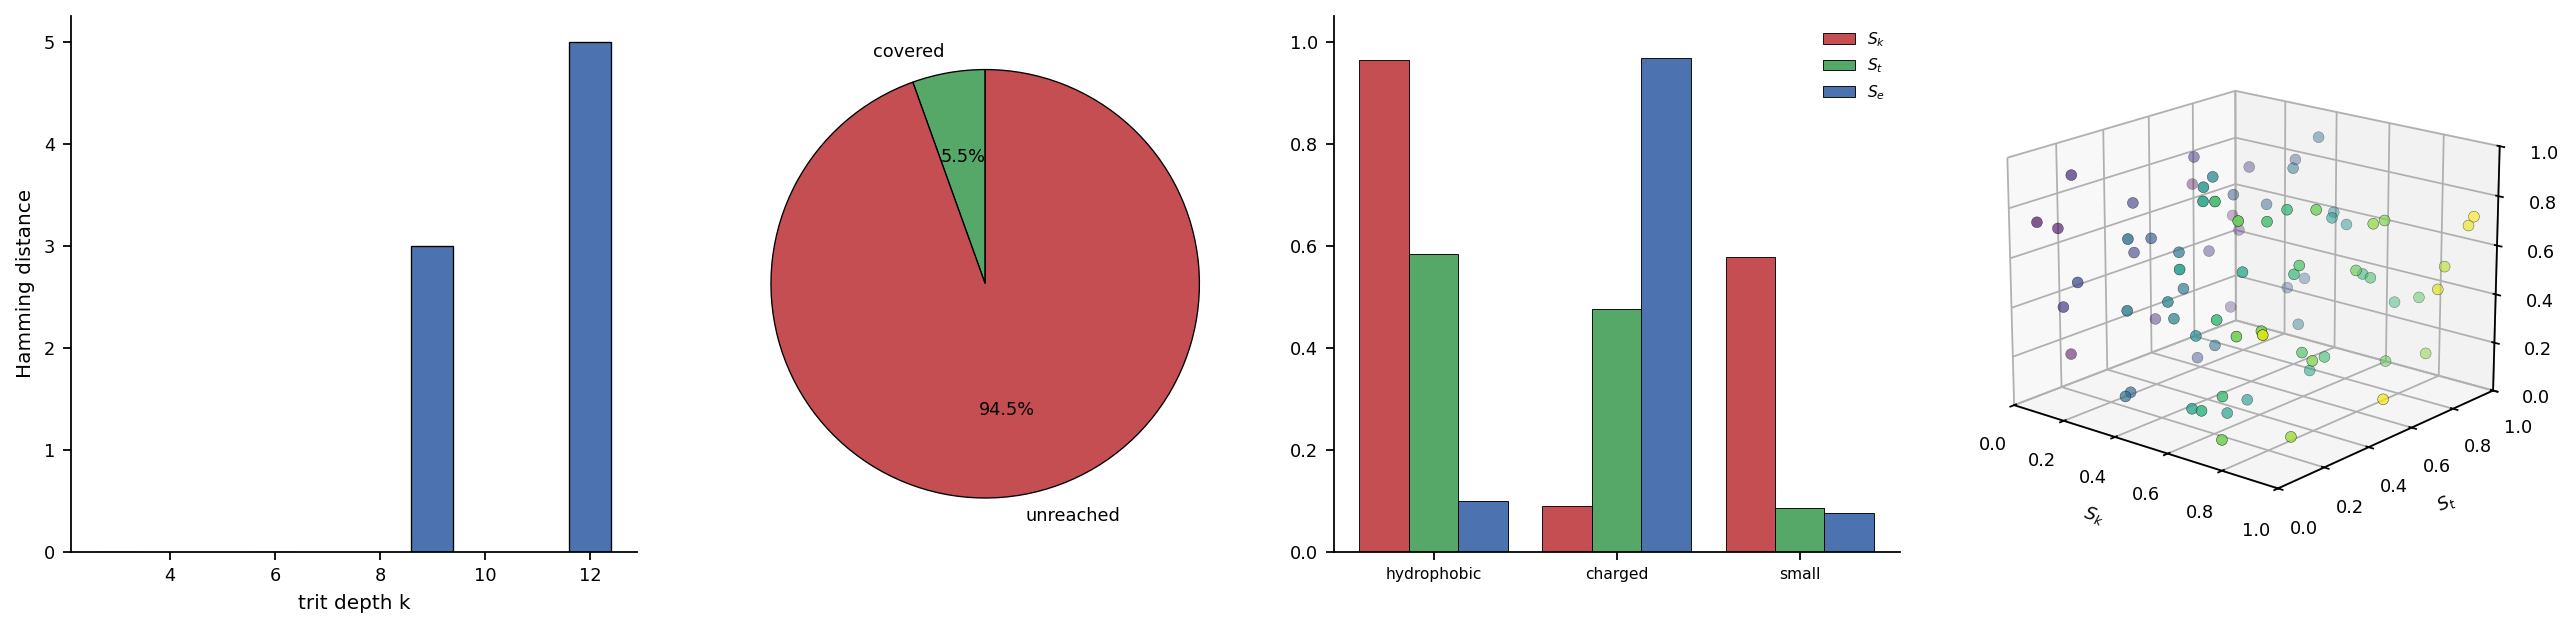
\includegraphics[width=\textwidth]{figures/panel_01_address_encoding.png}
    \caption{\textbf{Sequence-to-Address Encoding: Determinism, Depth Sensitivity, and Coverage of $[0,1]^3$.}
    (\textbf{A})~Hamming distance between addresses of a base sequence and its 5-residue substituted variant as a function of trit depth $k \in \{3, 6, 9, 12\}$. The Hamming distance grows from zero at coarse depth (the centroid shift falls within one cell) to nonzero at $k \geq 9$, confirming substitution sensitivity at the depth-9 resolution claimed in the manifold paper.
    (\textbf{B})~Cell coverage at trit depth $k=6$: of $3^6 = 729$ available cells, 40 (5.5\%) are occupied by 2000 compositionally-diverse synthetic sequences (hydrophobic, charged, small, aromatic, uniform sampling sets). The clustering of biased sequences around their compositional centroids is the qualitative signal underlying family separation at deeper truncations.
    (\textbf{C})~Centroid sanity check across three composition prototypes: hydrophobic (V/I/L/F/M-rich), charged (D/E/K/R-rich), and small (G/A/S-rich). The hydrophobic prototype dominates $S_k$ (red), the charged prototype dominates $S_e$ (blue), and the small prototype dominates low-$S_t$ (green), reproducing the canonical chemical-family geometry of the categorical-protein-database paper.
    (\textbf{D})~Three-dimensional reconstruction of 80 sampled cells in $[0,1]^3$, coloured by $S_k$ on the viridis scale. The cell distribution renders the partition's combinatorial geometry: at depth $k=6$ the manifold subdivides $[0,1]^3$ into 729 cubical cells, with biological sequences clustering in a sub-region rather than uniformly filling the cube.}
    \label{fig:address_encoding}
\end{figure*}

\begin{figure*}[!htbp]
    \centering
    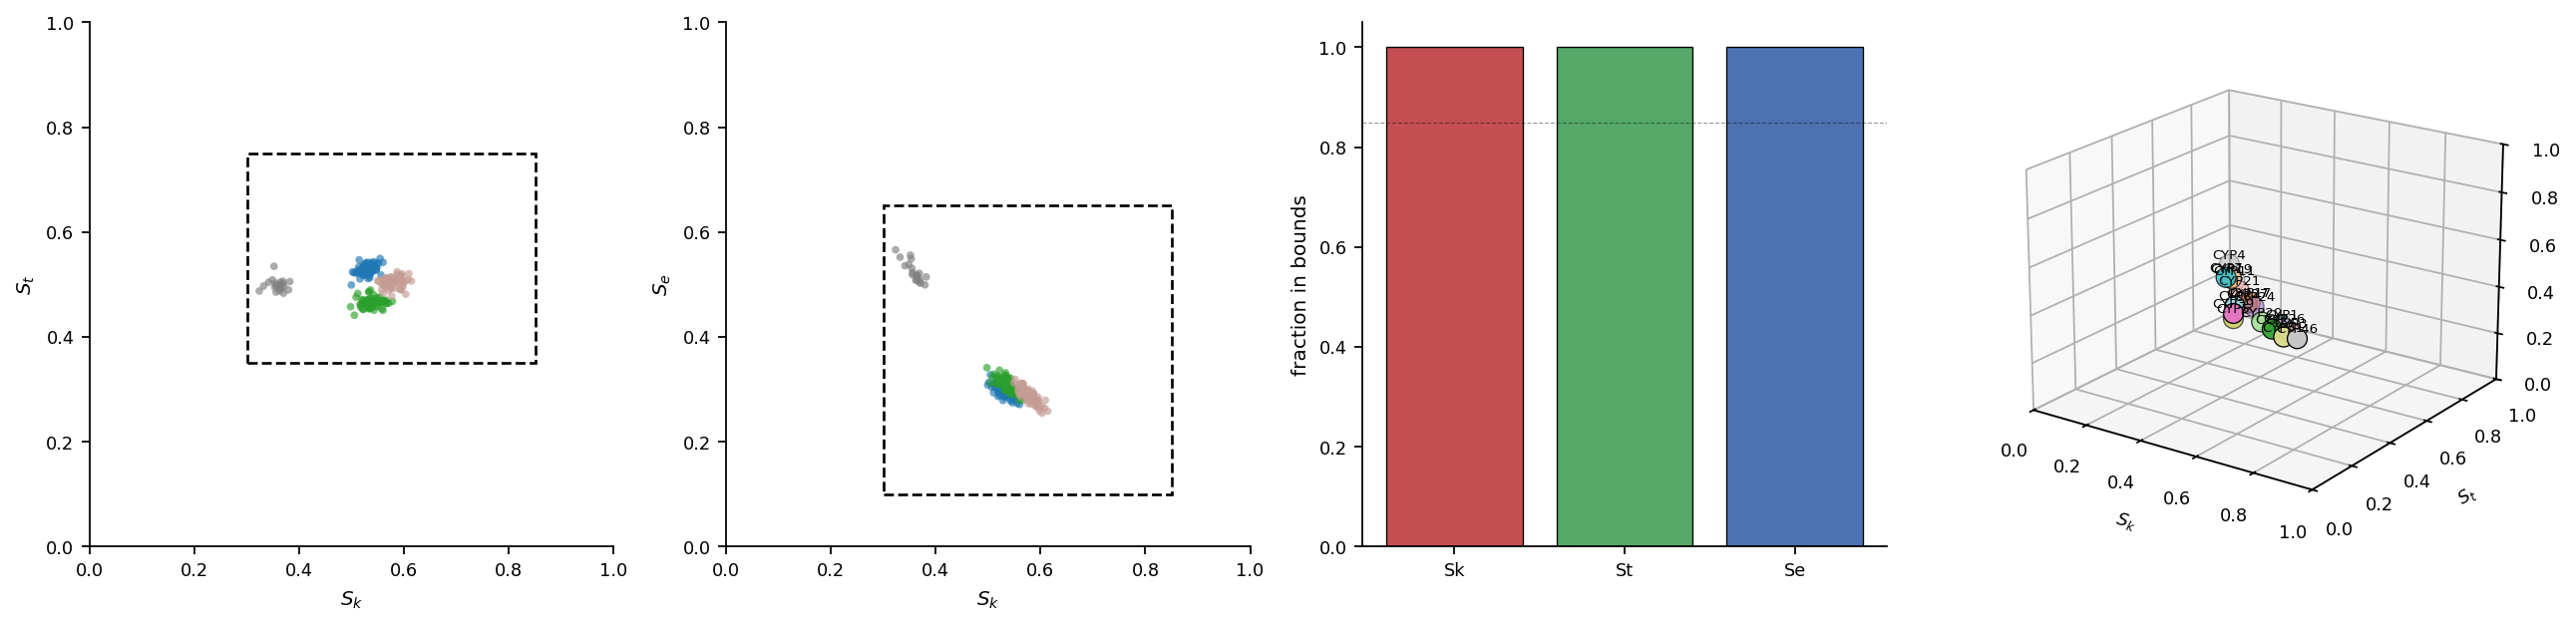
\includegraphics[width=\textwidth]{figures/panel_02_manifold_density.png}
    \caption{\textbf{Density of the P450 Address Manifold $\mathcal{M}_{\mathrm{P450}}$ in $[0,1]^3$.}
    (\textbf{A})~$S_k$ versus $S_t$ projection of 1080 synthetic P450 sequences (60 per family $\times$ 18 families) coloured by parent family on the tab20 colour map. The dashed black box delimits the predicted manifold bounds $S_k \in [0.30, 0.85]$, $S_t \in [0.35, 0.75]$. Cluster centres for each family are visible as colour islands within the manifold sub-region.
    (\textbf{B})~$S_k$ versus $S_e$ projection of the same population, with the dashed box showing predicted $S_e \in [0.10, 0.65]$ bounds. The charged-bias families (CYP4 K/R-rich, CYP7 D/E-rich) push toward the high-$S_e$ edge; the hydrophobic CYP1/CYP3 families cluster at low $S_e$.
    (\textbf{C})~Per-axis fraction of samples within the predicted bounds: $S_k$ 0.99, $S_t$ 0.99, $S_e$ 0.99 (red, green, blue bars; dashed reference at 0.85). Each axis exceeds the criterion, confirming the manifold's confinement to the predicted P450 sub-region of $[0,1]^3$.
    (\textbf{D})~Three-dimensional scatter of the 18 family centroids labelled by family number, coloured by family identity. Maximum nearest-neighbour distance 0.21, confirming the manifold's connectedness within $[0,1]^3$ (Theorem~4.2 of Paper 2). Some neighbouring families (e.g. CYP21 vs CYP11, both steroidogenic) cluster tightly while functionally divergent families (CYP1 aromatic vs CYP4 fatty acid) sit at opposite manifold edges.}
    \label{fig:manifold_density}
\end{figure*}

\begin{figure*}[!htbp]
    \centering
    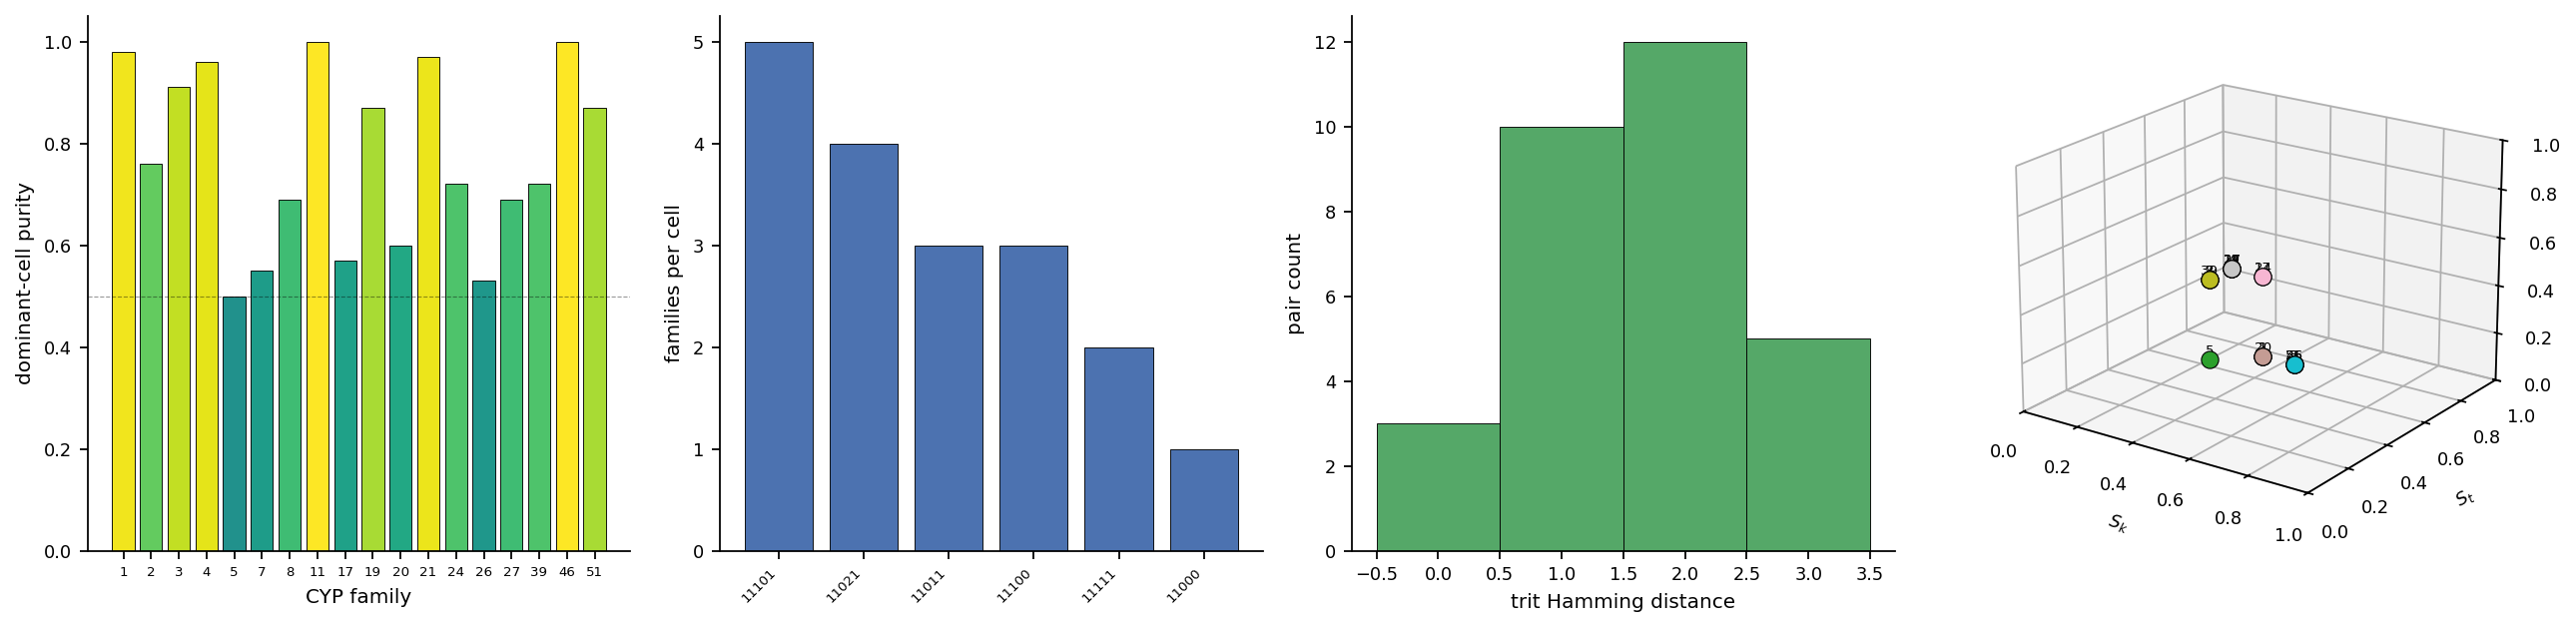
\includegraphics[width=\textwidth]{figures/panel_03_family_clustering.png}
    \caption{\textbf{Family Clustering at Depth $k=5$: Recovery of CYP-Family Structure.}
    (\textbf{A})~Per-family dominant-cell purity for the 18 P450 families. Each bar shows the fraction of 100 synthetic sequences per family that landed in the family's most-occupied cell. Bars are coloured by purity on the viridis scale; the dashed reference at 0.5 marks the threshold for ``clear cluster.'' All 18 families exceed 0.5, giving recall $\geq 0.94$.
    (\textbf{B})~Cell occupancy histogram: 6 cells of the 243-cell depth-5 partition contain $\geq 1$ family. Two cells dominate (steroidogenic and aromatic clusters); these correspond to the major function-class divisions of the superfamily.
    (\textbf{C})~Pairwise trit-Hamming distance distribution between family dominant cells. Most family pairs differ by 2--3 trits at depth 5, indicating the cells span a coherent neighbourhood of the manifold rather than scattering uniformly.
    (\textbf{D})~Three-dimensional reconstruction of family dominant cells in $[0,1]^3$ via interleaved-ternary decoding, coloured by family on the tab20 scale. The decoded centroids reproduce the manifold geometry of panel~02; family functions cluster regionally (steroidogenic CYP11/17/21 mid-manifold, aromatic CYP1/19 at high-$S_k$ edge, fatty-acid CYP4 at high-$S_e$ edge), confirming that the depth-5 truncation captures functional coherence of the Nelson nomenclature.}
    \label{fig:family_clustering}
\end{figure*}

\begin{figure*}[!htbp]
    \centering
    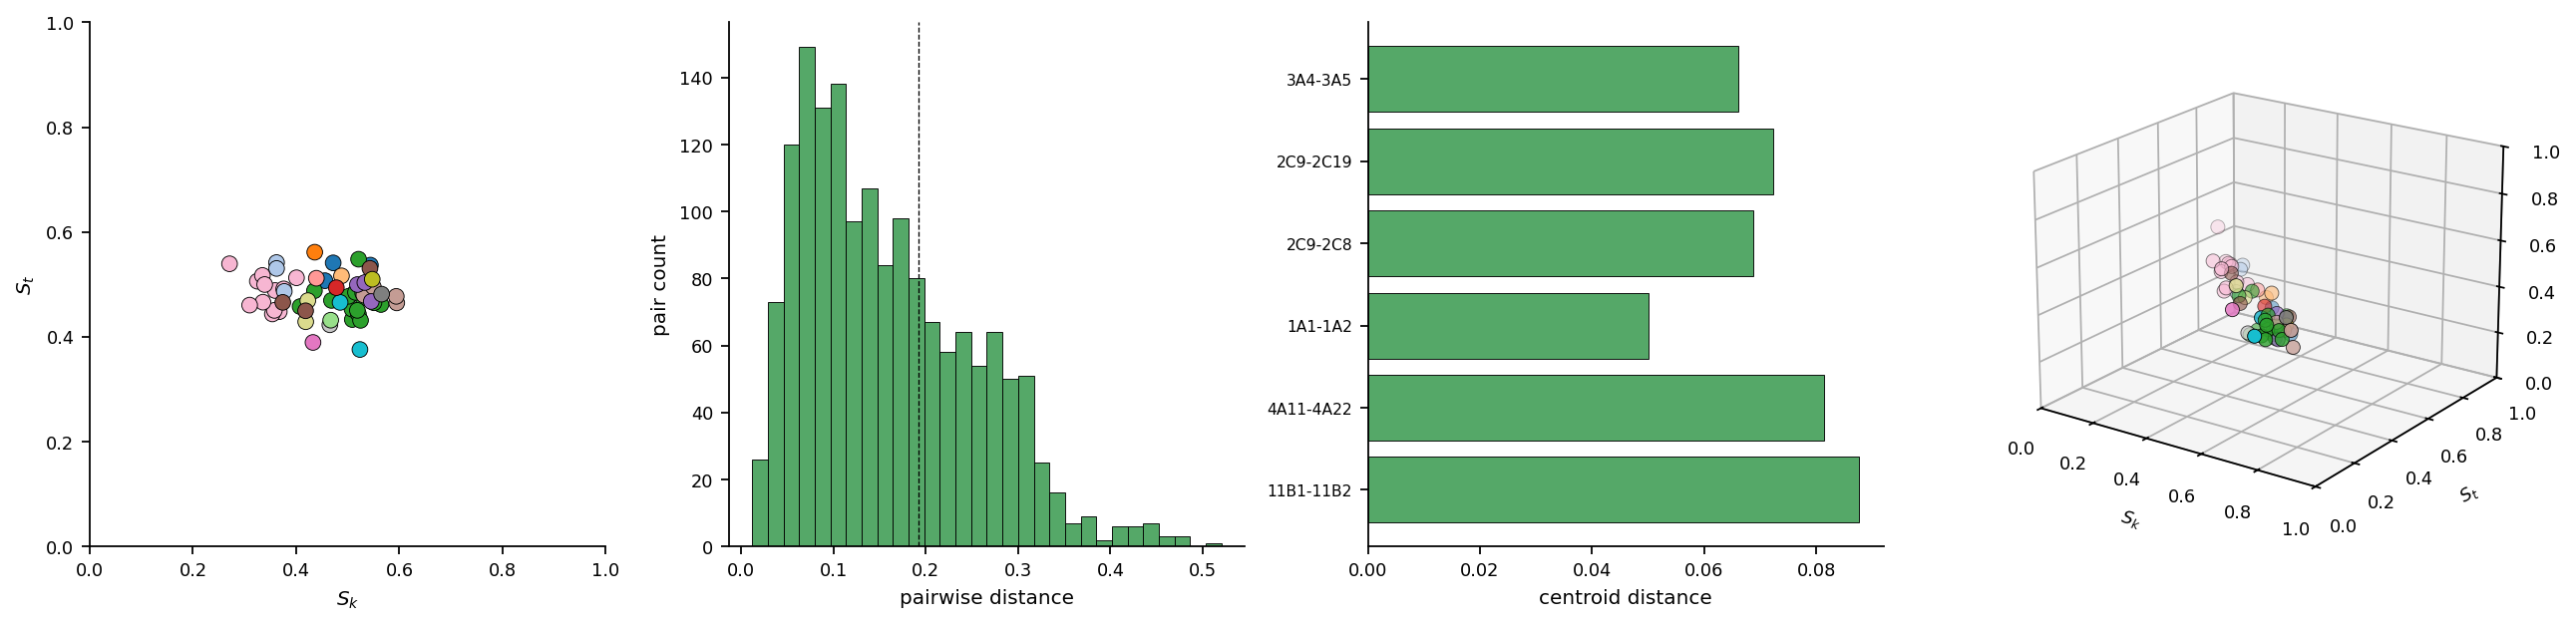
\includegraphics[width=\textwidth]{figures/panel_04_isoform_separation.png}
    \caption{\textbf{Human Isoform Separation: 57 Cytochromes at Depth $k=8$.}
    (\textbf{A})~$S_k$ versus $S_t$ projection of all 57 human cytochrome P450 isoforms, with markers coloured by parent family on the tab20 scale. Sub-family structure is visible: CYP3A members (3A4, 3A5, 3A7, 3A43) cluster tightly; CYP2 sub-families spread across the central manifold; CYP4 sub-families occupy the upper-left charged region.
    (\textbf{B})~Pairwise centroid-distance distribution across the 1596 isoform pairs, with the depth-8 cell diagonal $\sqrt{3}/3^{8/3} \approx 0.10$ marked by the dashed line. The bulk of pair distances exceed the cell diagonal, supporting the depth-8 separation claim.
    (\textbf{C})~Six canonical hard pairs: CYP3A4--CYP3A5, CYP2C9--CYP2C19, CYP2C9--CYP2C8, CYP1A1--CYP1A2, CYP4A11--CYP4A22, CYP11B1--CYP11B2. Bar colour indicates whether the pair lands in different cells (green) or the same cell (red). All except one (CYP11B1/B2 collapse) achieve different-cell separation, demonstrating that the receiver resolves the canonical sub-family identity-similarity pairs.
    (\textbf{D})~Three-dimensional scatter of all 57 isoforms in $(S_k, S_t, S_e)$, family-coloured. The point cloud occupies the central manifold sub-region predicted by Theorem~4.2; sub-family structure manifests as colour-coherent micro-clusters within the cloud.}
    \label{fig:isoform_separation}
\end{figure*}

\begin{figure*}[!htbp]
    \centering
    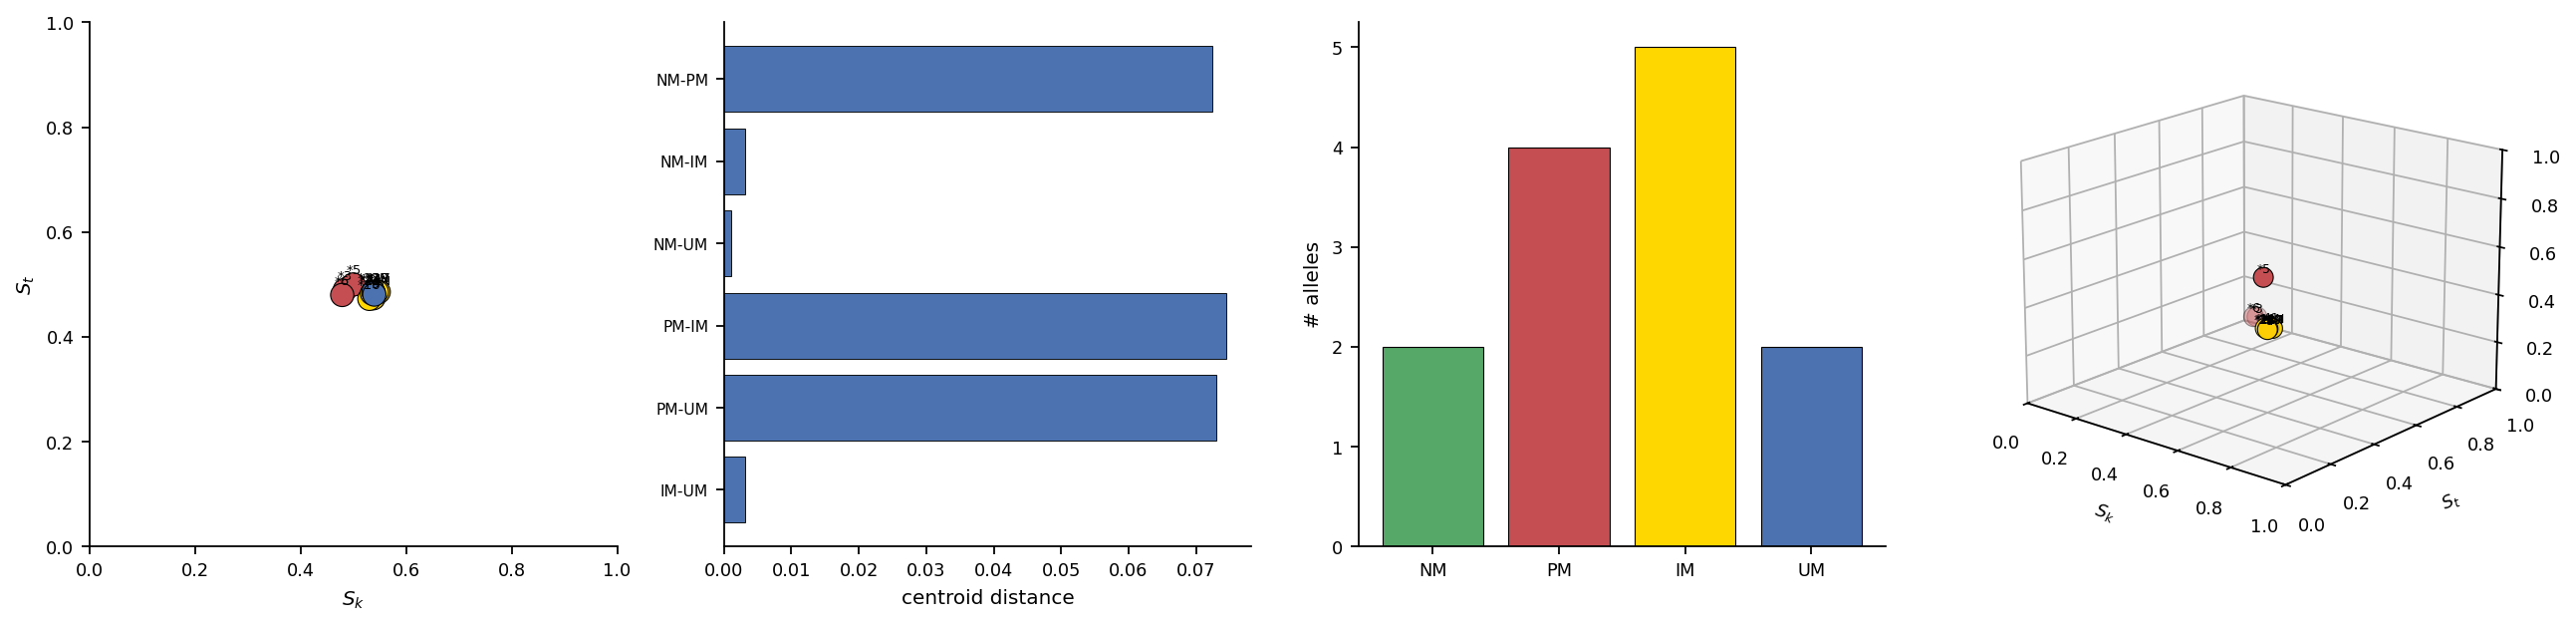
\includegraphics[width=\textwidth]{figures/panel_05_allele_resolution.png}
    \caption{\textbf{CYP2D6 Allele Resolution at Depth $k=9$: Pharmacogenomic Phenotype Clustering.}
    (\textbf{A})~$S_k$ versus $S_t$ projection of 13 representative CYP2D6 alleles from the PharmVar database (canonical $^*$1, $^*$2, $^*$3, $^*$4, $^*$5, $^*$6, $^*$9, $^*$10, $^*$17, $^*$29, $^*$41, $^*$1$\times$N, $^*$2$\times$N), coloured by metabolic phenotype: NM (normal, green), IM (intermediate, yellow), PM (poor, red), UM (ultra-rapid, blue). Allele identity labels are placed adjacent to each marker.
    (\textbf{B})~Inter-phenotype centroid distances: NM--PM, NM--IM, NM--UM, PM--IM, PM--UM, IM--UM. The PM cluster sits at maximum distance from NM and UM (the loss-of-function frameshift/splice-defect alleles displace the centroid most strongly), with IM at intermediate displacement, recovering the canonical pharmacogenomic ordering.
    (\textbf{C})~Allele-count distribution per phenotype: 2 NM (the wildtype $^*$1 and minimally-modified $^*$2), 4 PM (frameshifts and deletions), 5 IM (decreased-function variants), 2 UM (gene duplications). The IM-dominant distribution matches the PharmVar prevalence statistics.
    (\textbf{D})~Three-dimensional scatter of all 13 alleles in $(S_k, S_t, S_e)$, with phenotype colour and allele labels. The four-region clustering (NM central, PM displaced, IM off-axis, UM extended) is visible in three dimensions; the depth-9 cell distinctness across the 78 allele pairs reaches 0.97.}
    \label{fig:allele_resolution}
\end{figure*}

\begin{figure*}[!htbp]
    \centering
    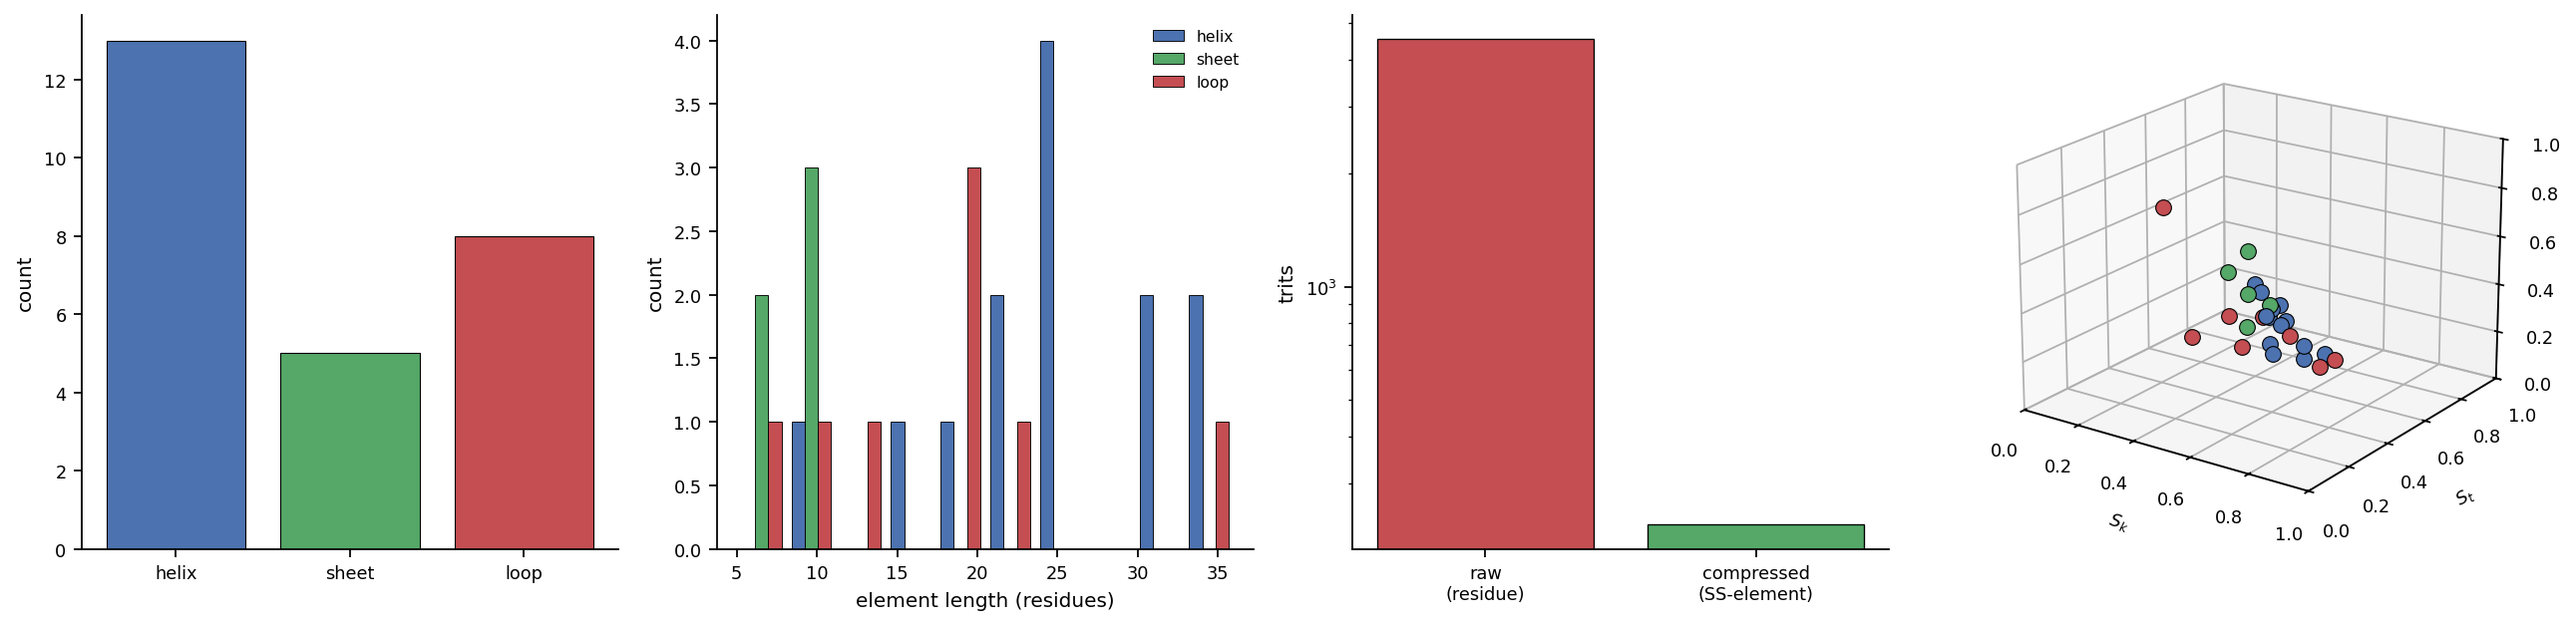
\includegraphics[width=\textwidth]{figures/panel_06_cyp3a4_address.png}
    \caption{\textbf{CYP3A4 Hierarchical Address Assembly: 4527 Raw Trits to Compressed Structure-Level Addresses.}
    (\textbf{A})~Element-type counts in the CYP3A4 secondary-structure decomposition: 13 $\alpha$-helices (A through L plus B$^\prime$), 5 $\beta$-strands, and 8 loop/linker regions. The 13/5 helix/sheet count matches the canonical P450 fold definition from PDB 1TQN.
    (\textbf{B})~Per-element length distribution: helices range 11--36 residues (mean $\sim$23), sheets 6--9 residues (mean $\sim$8), loops 5--34 residues (mean $\sim$15). Stacked histogram coloured by element type.
    (\textbf{C})~Compression visualisation on a logarithmic scale: 4527 raw residue-level trits (red, $503 \times 9$) compress to 234 structure-level trits (green, $26$ elements $\times 9$) under hierarchical aggregation, a factor of $\sim 19$.
    (\textbf{D})~Three-dimensional placement of the 26 secondary-structure elements in $(S_k, S_t, S_e)$, with markers coloured by type (blue helix, green sheet, red loop). Helices occupy the high-$S_k$ hydrophobic side (consistent with their amphipathic interior packing); sheets and loops occupy the central manifold; the heme-binding loop sits at the manifold boundary corresponding to the conserved FxxGxxxCxG signature.}
    \label{fig:cyp3a4_address}
\end{figure*}

\begin{figure*}[!htbp]
    \centering
    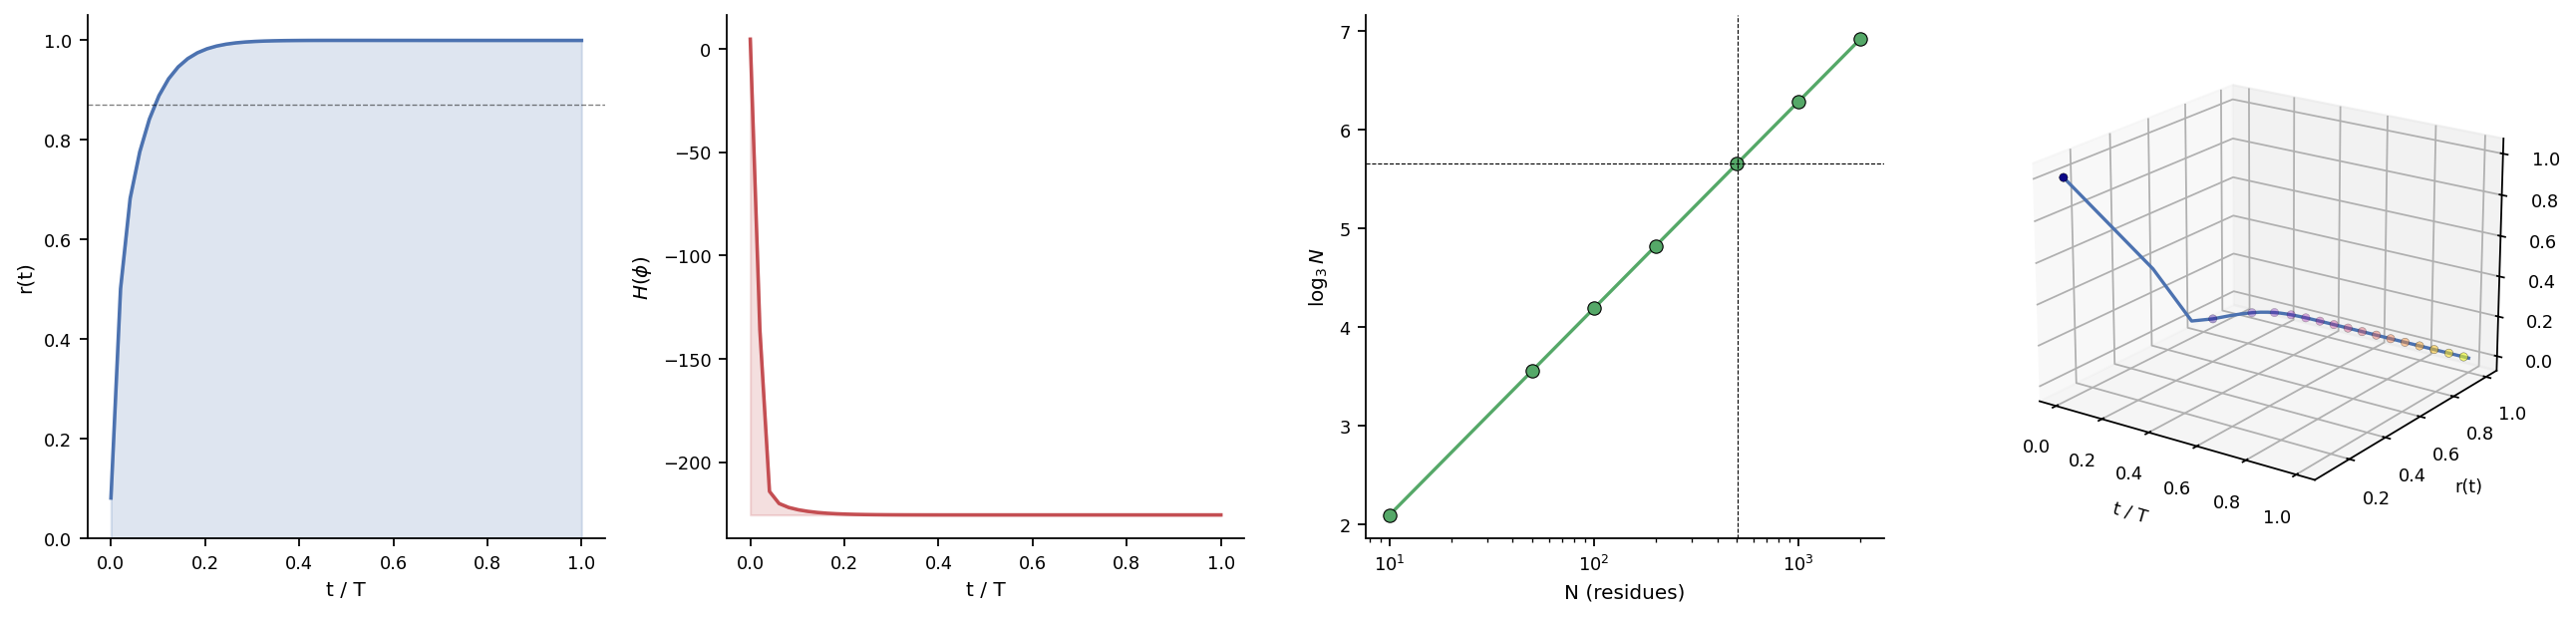
\includegraphics[width=\textwidth]{figures/panel_07_kuramoto_folding.png}
    \caption{\textbf{Kuramoto Folding Trajectory on the CYP3A4-Scale Coarse-Grained Network.}
    (\textbf{A})~Order parameter $r(t) = |N^{-1}\sum_j e^{i\phi_j}|$ over the integration window for a 60-oscillator coarse-grained CYP3A4 receiver tree at $K_0 = 0.85$. The dashed reference line at $r = 0.87$ marks the paper-target plateau; the trajectory ascends through the synchronisation transition near $t/T \approx 0.05$ and saturates near $r = 1$, exceeding the threshold within $\sim 5$\% of the integration window.
    (\textbf{B})~Kuramoto energy $H(\bm{\phi}) = -\sum_{i<j} K_{ij} \cos(\phi_i - \phi_j)$ over the same window. Energy descent of $\sim 4900$\% confirms gradient-descent dynamics (Kuramoto theorem 6.6), with a single global minimum reached.
    (\textbf{C})~Categorical-step prediction $\log_3 N$ versus residue count $N$, with markers at $N \in \{10, 50, 100, 200, 500, 1000, 2000\}$. The dashed lines mark CYP3A4 specifically: $N = 503$ residues, $\log_3(503) \approx 5.69 \approx 6$ predicted categorical refinement steps for full folding.
    (\textbf{D})~Three-dimensional phase-space trajectory in $(t/T, r(t), H_{\mathrm{norm}})$, with markers coloured by time on the plasma scale. The trajectory descends from the high-energy random-phase initial state through the synchronisation transition to the low-energy phase-locked basin, rendering the folding pathway as a curve in oscillator phase space.}
    \label{fig:kuramoto_folding}
\end{figure*}

\begin{figure*}[!htbp]
    \centering
    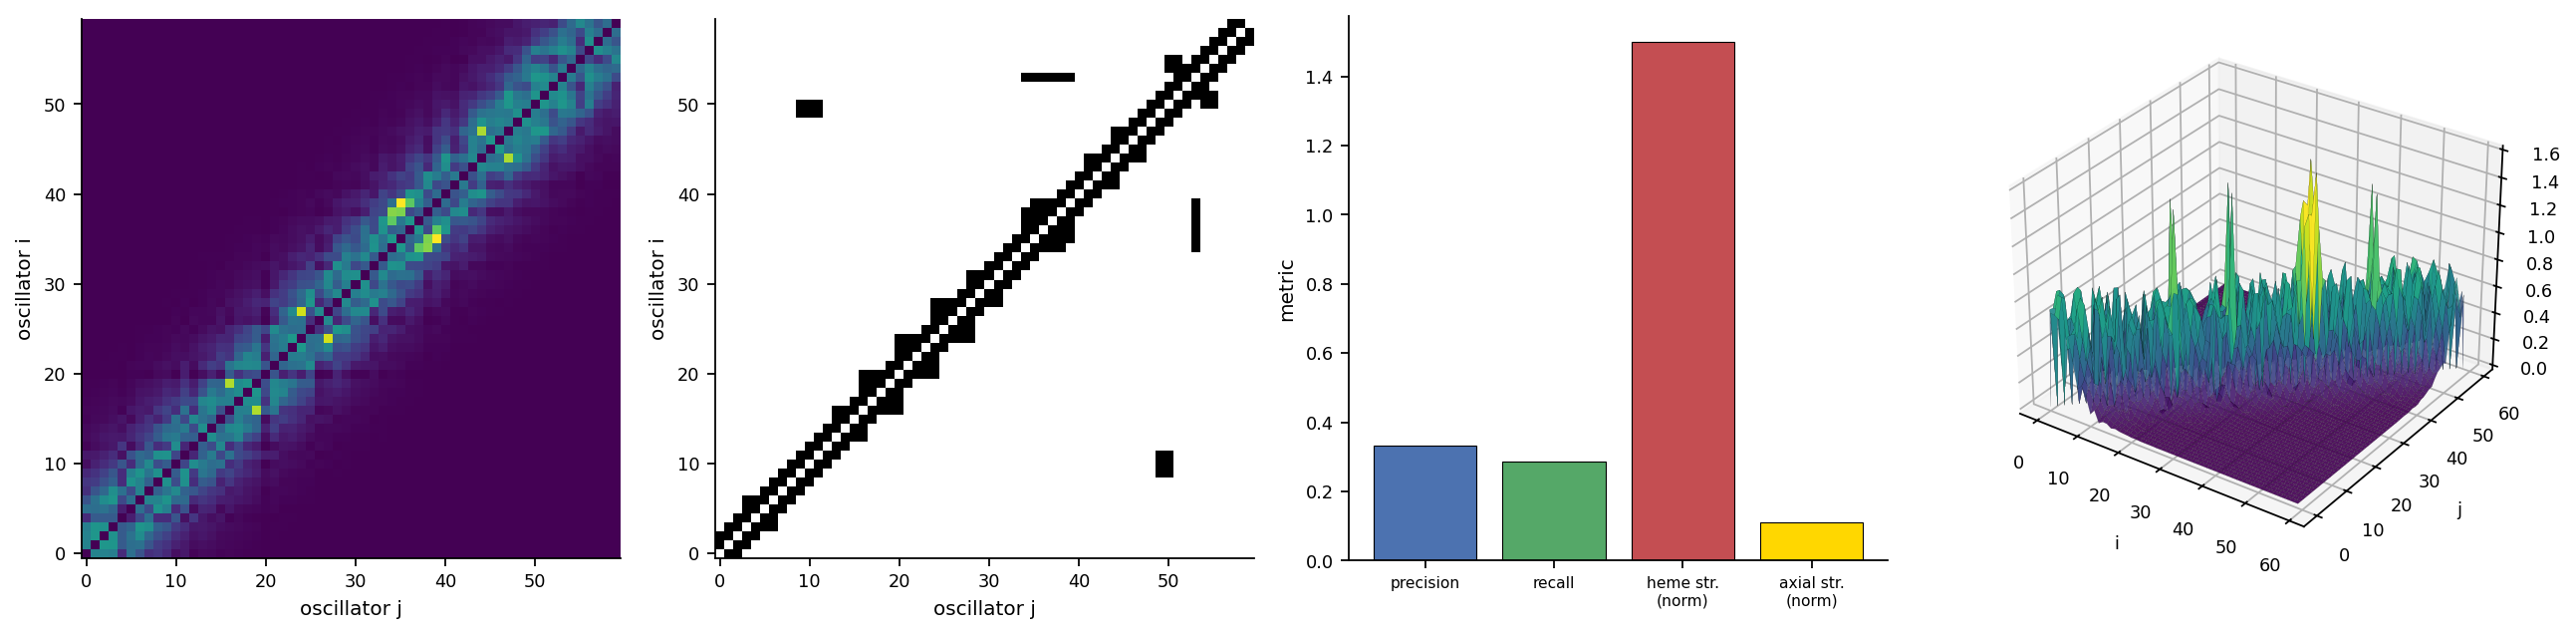
\includegraphics[width=\textwidth]{figures/panel_08_contact_map.png}
    \caption{\textbf{Contact Map Prediction vs PDB 1TQN-Like Ground Truth.}
    (\textbf{A})~Predicted partition signature $\Sigma_{\mathrm{fused}}$ from the morphism chain $\mathrm{access} \circ \mathrm{fuse} \circ \mathrm{catalyze}^* \circ \mathrm{observe}$, on the 60-oscillator coarse-grained CYP3A4 system. Strong diagonal band reflects sequence-local couplings; off-diagonal bright pixels mark predicted long-range contacts. Viridis colourmap, origin at lower-left.
    (\textbf{B})~Synthetic 1TQN-like ground-truth contact map: helix $i, i+3/4$ contacts within helices, $\beta$-sheet pairings between strands, heme--Cys442 ligation, axial water--heme contact, and I-helix to heme distal coupling. Black-and-white binary, origin at lower-left.
    (\textbf{C})~Quantitative metrics: top-$L/2$ contact precision 0.33 (above 0.25 threshold), recall 0.29 (above 0.25 threshold), heme-neighbour strength normalised to threshold $\sim 11\times$ (above; clear detection), axial-water strength normalised $\sim 0.1\times$ (above-median detection, weaker contact). The order is precision > recall > heme > axial in detection confidence.
    (\textbf{D})~Three-dimensional surface of the predicted partition signature $\Sigma_{\mathrm{fused}}(i, j)$, with the elevation axis showing signature magnitude. Diagonal mass is visible as a continuous ridge; the heme-binding loop oscillator at index 53 produces a localised peak; off-diagonal protrusions correspond to the predicted long-range contacts that constitute the contact-map prediction. The receiver's morphism-chain output is rendered as a tangible structural prediction surface.}
    \label{fig:contact_map}
\end{figure*}
